%\documentclass[preprint,tightenlines,showpacs,showkeys,floatfix,
%nofootinbib,superscriptaddress,fleqn]{revtex4} 
\documentclass[tightenlines,floatfix,nofootinbib,superscriptaddress,fleqn]{revtex4} 
%\documentclass[aps,epsfig,tightlines,fleqn]{revtex4}
\usepackage{kotex}
\usepackage[HWP]{dhucs-interword}
\usepackage[dvips]{color}
\usepackage{graphicx}
\usepackage{bm}
%\usepackage{fancyhdr}
%\usepackage{dcolumn}
\usepackage{defcolor}
\usepackage{amsmath}
\usepackage{amsfonts}
\usepackage{amssymb}
\usepackage{amscd}
\usepackage{amsthm}
\usepackage[utf8]{inputenc}
%\pagestyle{fancy}

\begin{document}

\title{\Large 2022년 2학기 물리학 II}
\author{Byeong-woo Han}
\email{12191964@inha.edu}
\author{김현철\footnote{Office: 5S-436D (면담시간 매주
    수요일-16:15$\sim$18:00)}} 
\email{hchkim@inha.ac.kr}
\affiliation{Hadron Theory Group, Department of Physics,
  Inha University, Incheon 22212, Republic of Korea }
\date{Autumn Semester, 2022}

\maketitle

{\color{red} {\bf Due date:} 2022년 8월 31일  15:30-16:15 }
\vspace{1.cm}

\section*{\large Quiz 2}
\noindent {\bf 문제 1 [20pt].}
반지름이 $a$인 원형고리가 원점을 중심으로 $x-y$ 평면에 놓여 있다.  
이 중심에서부터 $z$축으로 $z$만큼 떨어진 $P$점에서 이 원형고리가
생성시키는 전기장의 크기와 방향을 구하려고 한다.
\begin{itemize}
\item 원점에서부터 원형고리를 따라 있는 미소길이 $ds$까지의 거리 벡터
  $\vec{r}'$을 구하여라. 
\item 원점에서부터 $P$점까지 거리 벡터 $\vec{r}$을 구하여라.
\item $|\vec{r}-\vec{r}'|$을 구하여라. 
\item 위 문제에 대한 전기장을 표현하여라. 
\item $P$점에서 전기장을 구하여라. 
\item 결과를 토론하여라. (예: 전기장의 방향은 왜 $z$축 방향만 있는가?
  $z\gg a$ 일 때 전기장은? 등등)  
\end{itemize}
\vspace{1.cm}
\noindent {\bf 풀이 :}
 \begin{figure}[htp]
   \centering
   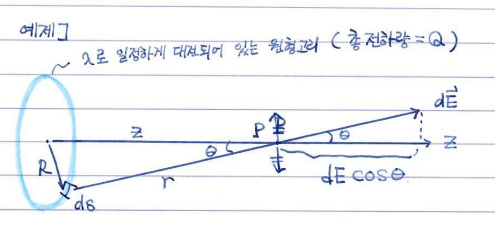
\includegraphics[scale=1]{problem 1.png}
   \caption{\textbf{문제 1}}
   \label{fig:1}
 \end{figure}
먼저 미소거리 $ds$까지의 거리 벡터$\vec{r}'$을 구해보자.
$ds$까지의 거리벡터 $\vec{r}'$와 $x$축과의 각도를 $\phi$라고 하자.
그러면 $\vec{r}'$을 다음과 같이 쓸 수 있다.
\begin{align}
  \vec{r}'=\left(a\cos{\phi},a\sin{\phi},0\right).
\end{align}
  또한, 원점에서 $P$점까지의 거리 벡터 $\vec{r}$ 역시 쉽게 쓸 수 있다.
\begin{align}
  \vec{r}=\left(0,0,z\right).
\end{align}
따라서, $\left|\vec{r}-\vec{r}'\right|$은 다음과 같다.
\begin{align}
  &\left|\vec{r}-\vec{r}'\right|=\left|\left(-a\cos{\phi},-a\sin{\phi},z\right)\right|\\
  =&\sqrt{a^2\cos^2{\phi}+a^2\sin^2{\phi}+z^2}.
\end{align}
$\sin^2{\phi}+\cos^2{\phi}=1$이므로,
\begin{align}
  &\left|\vec{r}-\vec{r}'\right|=\sqrt{a^2+z^2}
\end{align}
이다. 이제 전기장을 표현하기 위하여 전하를 알아보자.
전하밀도가 균일하므로 전하밀도는 상수이다. 이 전하밀도를 $\lambda$라고 하자.
전체 전하를 $Q$라고 하였을 때 $\lambda$와 $Q$사이의 관계는 다음과 같다.
\begin{align}
  \lambda=\frac{Q}{2\pi a}.
\end{align}
이제 미소길이 $ds$에 의한 미소 전기장을 구해보자. $ds$에 의한 전기장은 다음과 같이 표현 될 수 있다.
\begin{align}
  d\vec{E}=\frac{1}{4\pi \epsilon_0}\frac{dq}{\left|\vec{r}-\vec{r}'\right|^3}\left(\vec{r}-\vec{r}'\right).
\end{align}
여기서 $dq=\lambda ds=\frac{Q}{2\pi a} a d\phi$ 이고, $\left|\vec{r}-\vec{r}'\right|$과 $\left(\vec{r}-\vec{r}'\right)$는 이미 구했으므로
미소 전기장에 대한 식은 쉽게 알 수 있다.
\begin{align}
  d\vec{E}=\frac{1}{4\pi \epsilon_0}\frac{Q}{2\pi a}\frac{a}{\left(a^2+z^2\right)^{3/2}}\left(-a\cos{\phi}\hat{x}-a\sin{\phi}+z\hat{z}\right)d \phi.
\end{align}
이제 총 전기장을 구하기 위해 $0$부터 $2\pi$까지 적분하자.
\begin{align}
  \vec{E}&=\int^{2\pi}_{0}\frac{1}{4\pi \epsilon_0}\frac{Q}{2\pi a}\frac{a}{\left(a^2+z^2\right)^{3/2}}\left(-a\cos{\phi}\hat{x}-a\sin{\phi}\hat{y}+z\hat{z}\right)d\phi\\
  &=\frac{1}{4\pi \epsilon_0}\frac{Q}{2\pi}\frac{1}{\left(a^2+z^2\right)^{3/2}}\left(-a\sin{\phi}\hat{x}+a\cos{\phi}\hat{y}+\phi z\hat{z}\right)|^{2\pi}_0 \\
  &=\frac{1}{4 \pi \epsilon_0}\frac{Qz}{\left(a^2+z^2\right)^{3/2}}\hat{z}.
\end{align}
이다. 강의노트에서는 대칭성이 존재함을 전제로 하여서 $\cos$성분만 이용하여서 전기장을 구하였지만
여기에서의 풀이과정에서는 벡터의 방향을 모두 고려하여 계산을 하였다. 그럼에도 불구하고 같은결과가 나왔는데, 이러한 결과가 나온 이유는 언급하였다 싶이 원이 원점을 기준으로 $z$축에 대한 대칭성이 존재하기 때문이다.
또한 만약에 $z \gg a$일 때 전기장을 구해보면, $1\gg \frac{a}{z}$ 이므로, Taylor근사가 가능하다. 따라서,
\begin{align}
  \begin{split}
    \vec{E}&=\frac{1}{4 \pi \epsilon_0}\frac{Qz}{\left(a^2+z^2\right)^{3/2}}\hat{z}\\
    &=\frac{1}{4 \pi \epsilon_0}\frac{Qz}{z^3\left[1+\left(\frac{a}{z}\right)^2\right]^{3/2}}\hat{z}\\
    &=\frac{1}{4 \pi \epsilon_0}\frac{Q}{z^2}\left[1+\left(\frac{a}{z}\right)^2\right]^{-3/2}\hat{z}\\
    &\approx\frac{1}{4 \pi \epsilon_0}\frac{Q}{z^2}\left(1-\frac{3}{2}\frac{a^2}{z^2}\right)\hat{z}\\
    &=\frac{1}{4 \pi \epsilon_0}\frac{Q}{z^2}\hat{z}+O\left(\frac{a^2}{z^4}\right)\hat{z}\\
    &\approx\frac{1}{4 \pi \epsilon_0}\frac{Q}{z^2}\hat{z}
  \end{split}
\end{align}
를 얻는다. 따라서, $z \gg a$일 때, 전하밀도가 일정한 원형고리는 점전하로 근사가 가능하다.\\
이제 $z\rightarrow 0$일때의 전기장을 구해보자. 이떄의 전기장은,
\begin{align}
  \lim_{z\rightarrow 0}\frac{1}{4 \pi \epsilon_0}\frac{Qz}{\left(a^2+z^2\right)^{3/2}}\hat{z}=\vec{0}
\end{align}
이므로, $z=0$ 일 때, 전기장은 $\vec{0}$이다. 이러한 이유는 원의 중심에서 원의 대칭성에 의해서
전기장이 서로 상쇄되기 때문에, 전기장이 $\vec{0}$이 되기 때문이다.
\vspace{1.cm}

\noindent {\bf 문제 2 [5pt].}크기가 $1.00\times 10^3~\mathrm{N/C}$인 균일한
전기장 안에 전자를 가만히 놓았다. 전자가 1.00 cm를 진행했을 때,
\begin{itemize}
\item[(가)] 전자의 속력은 얼마인가? 
\item[(나)] 전자의 운동에너지는 얼마인가? 
\item[(다)] 시간은 얼마나 지났는가? 
\end{itemize}
\vspace{1.cm}
\noindent {\bf 풀이 :}
\begin{itemize}
\item[(가)] 전자가 받는 힘은 $e\vec{E}$이므로 뉴턴의 제 2법칙에 의해
\begin{align}
  \vec{F}=m_e\vec{a}=e\vec{E}
\end{align}
전자의 가속도는 $\frac{e\vec{E}}{m_e}$로 일정하다.
여기서 $e$는 전자의 전하량, $\vec{E}$는 전기장, $m_e$는 전자의 질량이다.
이는 등가속도 운동이므로, 등가속도운동에서의 방정식 
\begin{align}
  2as=v^2-v_0^2
\end{align}
이 성립한다. 여기서 
\begin{align}
  \vec{a}=\frac{e\vec{E}}{m_e}=\frac{1.60 \times 10^{-19}\mathrm{C} \times 1.00 \times 10^3~\mathrm{N/C}}{9.11\times10^{-31}~\mathrm{kg}}=1.76\times10^{14}~\mathrm{m/s^2}
\end{align}
이고, 전자를 가만히 놓았다고 하였으므로, $v_0=0$, 마지막으로, $s=1.00~\mathrm{cm}=0.01~\mathrm{m}$이므로,
전자의 속력은,
\begin{align}
  v=\sqrt{2\times0.01~\mathrm{m}\times1.76\times10^{14}~\mathrm{m/s^2}}\approx1.88\times10^6~\mathrm{m/s}
\end{align}
이다.
\item[(나)] 
일-에너지 정리에 의해서, 전자에 가해진 일의 크기는 운동에너지의 변화량과 같다,
처음의 전자가 정지해 있었으므로, 가해진 일의 크기가 운동에너지 이다.
전자의 가해진 일의 크기는,
\begin{align}
  F\cdot s=e\vec{E}\cdot \vec{s}=(1.60\times10^{-19}~\mathrm{C})(1.00\times10^3~\mathrm{N/C}) (0.01~\mathrm{m})=1.60\times 10^{-18}~\mathrm{J}
\end{align}
이다.
\item[(다)]
등가속도 운동에서,
\begin{align}
  s=s_0+v_0t+\frac{1}{2}at^2
\end{align}
이다. 여기서, $s_0=0$으로 설정하고, 전자를 가만히 놓았다고 하였으므로, $v_0=0$이다.
따라서, 다음과 같이 쓸 수 있다.
\begin{align}
  s=\frac{1}{2}at^2
\end{align}
이를 변형하면,
\begin{align}
  t=\sqrt{\frac{2s}{a}}
\end{align}
이고, $s=0.01~\mathrm{m}, a=1.76\times10^{14}~\mathrm{m/s^2}$
이므로, 시간 $t$는
\begin{align}
  t=\sqrt{\frac{2\times0.01}{1.76\times10^{14}~\mathrm{m/s^2}}}=1.14\times10^{-16}s
\end{align}
이다.
\end{itemize}
\vspace{1.cm}


\noindent {\bf 문제 3 [10pt].} 그림~\ref{fig:1}처럼 각각 전하가 $q$,
$-q$인 두 입자가 전기 쌍극자를 이루고 있다. $x\gg a$일 때 $x$ 축
위에서 전기장 $E_x$를 구하여라. 
\begin{figure}[htp]
  \centering
  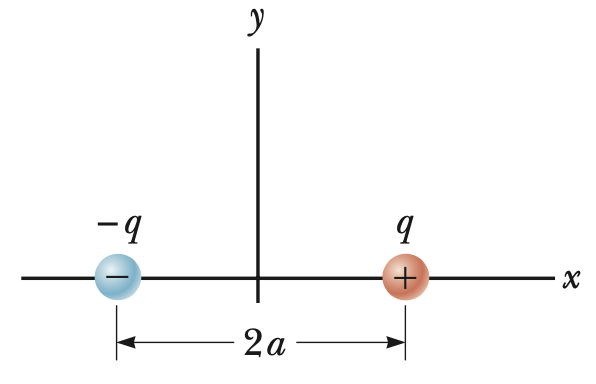
\includegraphics[scale=0.6]{qfig2-1.png}
  \caption{\textbf{문제 3}}
  \label{fig:1}
\end{figure}

\vspace{1.cm}
\noindent {\bf 풀이:}
먼저 양전하에 의한 전기장을 구하자. $x$축 위에서의 양전하에 의한 전기장 $E_q$는,
\begin{align}
  E_q=\frac{1}{4\pi\epsilon_0}\frac{q}{\left(x-a\right)^2}
\end{align}
이고, $x$축 위에서의 음전하에 의한 전기장 $E_{-q}$는,
\begin{align}
  E_{-q}=\frac{1}{4\pi\epsilon_0}\frac{-q}{\left(x+a\right)^2}
\end{align}
전기장은 중첩의 원리가 적용되므로, 중첩의 원리를 적용하면 전기장 $E_x$는
\begin{align}
  E_x=E_q+E_{-q}=\frac{1}{4\pi\epsilon_0}\frac{q}{\left(x-a\right)^2}+\frac{1}{4\pi\epsilon_0}\frac{-q}{\left(x+a\right)^2}
\end{align}
이제 $x\gg a$ 라고 가정하면, $1\gg\frac{a}{x}$ 이므로, Taylor 근사를 사용할 수 있다. 즉,
\begin{align}
  \begin{split}
    E_x&=\frac{1}{4\pi\epsilon_0}\frac{q}{x^2\left(1-\frac{a}{x}\right)^2}-\frac{1}{4\pi\epsilon_0}\frac{q}{x^2\left(1+\frac{a}{x}\right)^2}\\
    &=\frac{1}{4\pi\epsilon_0}\frac{q}{x^2}\left(1-\frac{a}{x}\right)^{-2}-\frac{1}{4\pi\epsilon_0}\frac{q}{x^2}\left(1+\frac{a}{x}\right)^{-2}\\
    &\approx\frac{1}{4\pi\epsilon_0}\frac{q}{x^2}\left[\left(1+\frac{2a}{x}\right)-\left(1-\frac{2a}{x}\right)\right]\\
    &=\frac{1}{4\pi\epsilon_0}\frac{4qa}{x^3}
  \end{split}
\end{align}
이다. 여기서 $p=2qa$라고 정의하면 $x$축 위의 전기장은 다음과 같이 쓸 수 있다.
\begin{align}
  E_x=\frac{1}{2\pi\epsilon_0}\frac{p}{x^3}
\end{align}
여기서의 $p$의 값을 쌍극자 모멘트라고 한다.
\vspace{1.cm}

\noindent {\bf 문제 4 [10pt].} 그림~\ref{fig:2}처럼 한 변의 길이가
$a$인 정사각형의 꼭짓점에 네 개의 전하가 각각 놓여있다.
\begin{figure}[htp]
  \centering
  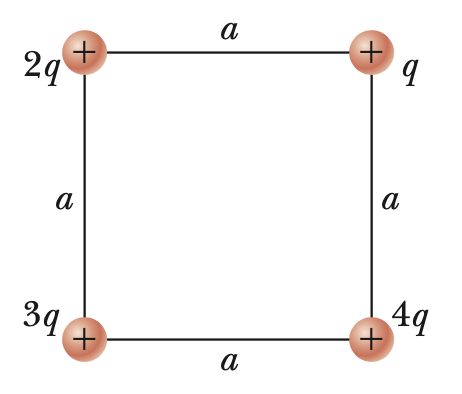
\includegraphics[scale=0.6]{qfig2-2.png}
  \caption{\textbf{문제 4}}
  \label{fig:2}
\end{figure}
\begin{itemize}
\item[(a)] 전하 $q$의 위치에서 전기장을 구하여라.
\item[(b)] $q$에 작용하는 총 정전기력을 구하여라.
\end{itemize}
\vspace{1.cm}
\noindent {\bf 풀이 :}
\begin{itemize}
  \item[(a)] 
  $q$에서의 전기장을 구하기 위해 $q,2q,3q,4q$에 의한 전기장을 구하자
  \item[(a-1)]
  $q$의 위치에서 $q$에 의한 전기장은, 거리가 $0$이므로, 전기장은 0이다
  \item[(a-2)]
  $q$의 위치에서 $2q$에 의한 전기장은 거리가 $a$이고, 방향이 $x$축 방향이므로,
  전기장 $\vec{E}_{2q}$는 다음과 같다.
  \begin{align}
    \vec{E}_{2q}=\frac{1}{4\pi\epsilon_0}\frac{2q}{a^2}\hat{x}.
  \end{align}
  \item[(a-3)]
  $q$의 위치에서 $3q$에 의한 전기장은 거리가 피타고라스 정리에 의해서
  $\sqrt{2}a$이고, $\hat{x}+\hat{y}$의 방향이므로, 전기장 $\vec{E}_{3q}$은 다음과 같다.
  \begin{align}
    \vec{E}_{3q}&=\frac{1}{4\pi\epsilon_0}\frac{3q}{2\sqrt{2}a^3}a\left(\hat{x}+\hat{y}\right)\\
    &=\frac{1}{4\pi\epsilon_0}\frac{3q}{2\sqrt{2}a^2}\left(\hat{x}+\hat{y}\right).
  \end{align}
  \item[(a-4)]
  $q$의 위치에서 $4q$에 의한 전기장은 $a$이고, 방향이 $y$축 방향이므로,
  전기장 $\vec{E}_{4q}$는 다음과 같다.
  \begin{align}
    \vec{E}_{4q}=\frac{1}{4\pi\epsilon_0}\frac{4q}{a^2}\hat{y}.
  \end{align}
  이다. 전기장은 중첩의 원리가 성립하므로, $q$의 위치에서의 전기장은
  다음과 같다.
  \begin{align}
    \begin{split}
      \vec{E}_{tot}&=\vec{E}_{2q}+\vec{E}_{3q}+\vec{E}_{4q}\\
      &=\frac{1}{4\pi\epsilon_0}\frac{2q}{a^2}\hat{x}+\frac{1}{4\pi\epsilon_0}\frac{3q}{2\sqrt{2}a^2}\left(\hat{x}+\hat{y}\right)+\frac{1}{4\pi\epsilon_0}\frac{4q}{a^2}\hat{y}\\
      &=\frac{1}{4\pi\epsilon_0}\frac{q}{a^2}\left(\frac{4\sqrt{2}+3}{2\sqrt{2}}\hat{x}+\frac{8\sqrt{2}+3}{2\sqrt{2}}\hat{y}\right).
    \end{split}
  \end{align}
  \item[(b)]
  전기장의 정의는 단위 전하당 전기력의 크기이다. 따라서, 총 정전기력은
  정의에 따라서 위에서 구한 전기장에 전하를 곱해주면 된다. 따라서 정전기력은
  \begin{align}
    \vec{F}_{tot}=q\vec{E}_{tot}=&=\frac{1}{4\pi\epsilon_0}\frac{q^2}{a^2}\left(\frac{4\sqrt{2}+3}{2\sqrt{2}}\hat{x}+\frac{8\sqrt{2}+3}{2\sqrt{2}}\hat{y}\right)
  \end{align}
  이다.
  \end{itemize}
\vspace{1.cm}

\noindent {\bf 문제 5 [20pt].} 
그림~\ref{fig:1}과 같이 $x$-축을 따라 두 전하 $q_1$과 $q_2$가 각각
$a$, $b$ 위치에 놓여 있다. 여기서 $q_2$는 음전하이다. 
\begin{itemize}
\item[(가)] $y$-축 위의 점 $P$에서 두 전하가 만드는 전기장을
  구하여라. 
\item[(나)] $|q_1|=|q_2|$, $a=b$일 때, $P$ 점에서 전기장을 구하여라. 
\item[(다)] 원점에서 $P$ 점까지의 거리가 $a$보다 매우 클 때 ($y\gg
  a$), 이 전기 쌍극자에 의한 전기장을 $P$ 점에서 구하여라. 
\end{itemize}
\begin{figure}[htp]
  \centering
  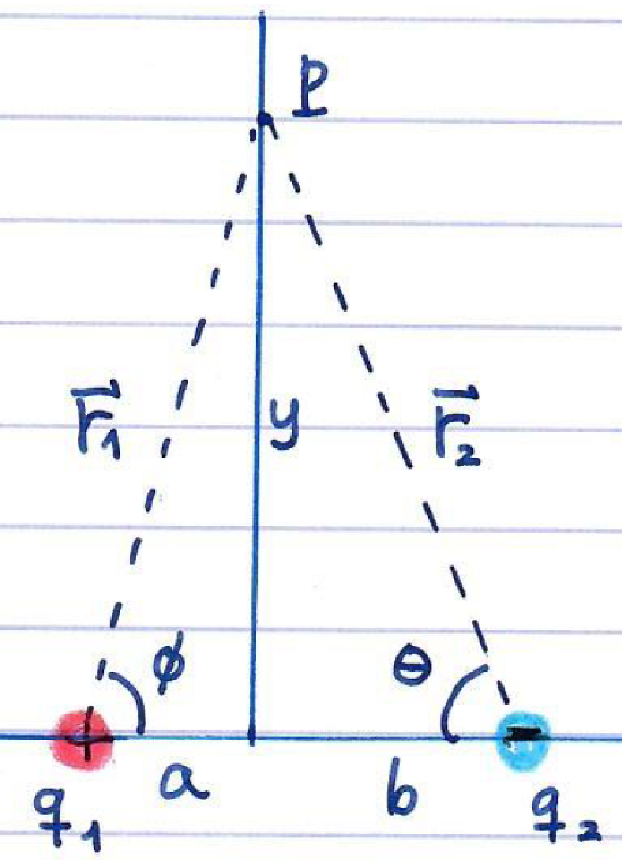
\includegraphics[scale=0.4]{Qfig20220829-1.pdf}
  \caption{\textbf{문제 5}}
  \label{fig:3}
\end{figure}
\vspace{1.cm}
\noindent {\bf 풀이 :}
\begin{itemize}
\item[(가)] 
  먼저 $q_1$이 만드는 점 P에서의 전기장 $\vec{E}_{q_1}$을 구하자. 이에 대한 식은 피타고라스의 정리를 이용하면 다음과 같다.
  \begin{align}\label{eq:5-1-1}
    \vec{E}_{q_1}=\frac{q_1}{4\pi\epsilon_0}\frac{1}{a^2+y^2}\frac{a\hat{x}+y\hat{y}}{\sqrt{a^2+y^2}}
  \end{align}
  같은 방법으로 $q_2$가 점 P에서 전기장 $\vec{E}_{q_2}$를 구해보면,
  \begin{align}\label{eq:5-1-2}
    \vec{E}_{q_2}=\frac{q_2}{4\pi\epsilon_0}\frac{1}{b^2+y^2}\frac{-b\hat{x}+y\hat{y}}{\sqrt{a^2+y^2}}
  \end{align}
  그런데 여기서 벡터부분을 삼각함수의 꼴로 변경할 수 있다. 즉,
  \begin{align}\label{eq:5-1}
    &\cos{\phi}=\frac{a}{\sqrt{a^2+y^2}}, \qquad \sin{\phi}=\frac{y}{\sqrt{a^2+y^2}},\\
    &\cos{\theta}=\frac{b}{\sqrt{b^2+y^2}}, \qquad \sin{\theta}=\frac{y}{\sqrt{b^2+y^2}} 
  \end{align}
  이다. 이 형태를 식~(\ref{eq:5-1-1}),~(\ref{eq:5-1-2})에 대입하여 다음과 같이 바꿔 쓸 수 있다.
  \begin{align}
    &\vec{E}_{q_1}=\frac{\left|q_1\right|}{4\pi\epsilon_0}\frac{1}{a^2+y^2}\left(\cos{\phi}\hat{x}+\sin{\phi}\hat{y}\right)\\
    &\vec{E}_{q_2}=\frac{\left|q_2\right|}{4\pi\epsilon_0}\frac{1}{b^2+y^2}\left(\cos{\theta}\hat{x}-\sin{\theta}\hat{y}\right).
  \end{align}
  따라서 점 P에서 두 전하가 만드는 전기장은,
  \begin{align}\label{eq:5-2}
    \begin{split}
      \vec{E}_{tot}&=\vec{E}_{q_1}+\vec{E}_{q_2}\\
      &=\frac{\left|q_1\right|}{4\pi\epsilon_0}\frac{1}{a^2+y^2}\left(\cos{\phi}\hat{x}+\sin{\phi}\hat{y}\right)+
      \frac{\left|q_2\right|}{4\pi\epsilon_0}\frac{1}{b^2+y^2}\left(\cos{\theta}\hat{x}-\sin{\theta}\hat{y}\right)\\
      &=\left(\frac{\left|q_1\right|}{4\pi\epsilon_0}\frac{1}{a^2+y^2}\cos{\phi}+\frac{\left|q_2\right|}{4\pi\epsilon_0}\frac{1}{b^2+y^2}\cos{\theta}\right)\hat{x}\\
      &+\left(\frac{\left|q_1\right|}{4\pi\epsilon_0}\frac{1}{a^2+y^2}\sin{\phi}-\frac{\left|q_2\right|}{4\pi\epsilon_0}\frac{1}{b^2+y^2}\sin{\theta}\right)\hat{y}
    \end{split}
  \end{align}
  이다.
\item[(나)] 
먼저 $a=b$인 경우를 생각하여 보자. 이 경우 식~(\ref{eq:5-1})에 의해서,
$\theta=\phi$가 된다. 또한, $\left|q_1\right|=\left|q_2\right|$ 까지 만족 할 경우,
식~(\ref{eq:5-2})에 의해서, y축 성분의 전기장이 사라지게 된다. 이때의 전하를
$\left|q_1\right|=\left|q_2\right|=\left|q\right|$이라고 한다면, 
$P$점에서의 전기장은
\begin{align}\label{eq:5-3}
  \begin{split}
    \vec{E}_{tot}&=\vec{E}_{q_1}+\vec{E}_{q_2}\\
    &=\left(\frac{\left|q\right|}{4\pi\epsilon_0}\frac{1}{a^2+y^2}\cos{\phi}+\frac{\left|q\right|}{4\pi\epsilon_0}\frac{1}{a^2+y^2}\cos{\phi}\right)\hat{x}\\
    &+\left(\frac{\left|q\right|}{4\pi\epsilon_0}\frac{1}{a^2+y^2}\sin{\phi}-\frac{\left|q\right|}{4\pi\epsilon_0}\frac{1}{a^2+y^2}\sin{\phi}\right)\hat{y}\\
    &=\frac{2\left|q\right|}{4\pi\epsilon_0}\frac{1}{a^2+y^2}\cos{\phi}\hat{x}\\
    &=\frac{2a\left|q\right|}{4\pi\epsilon_0}\frac{1}{\left(a^2+y^2\right)^{3/2}}\hat{x}
  \end{split}
\end{align}
이다.
\item[(다)]
	$y \gg a$ 라면, $1 \gg \frac{a}{y}$ 이므로 Taylor 근사를 쓸 수 있다.
  따라서, 식~(\ref{eq:5-3})을 다음과 같이 쓸 수 있다.
  \begin{align}
    \begin{split}
      \vec{E}_{tot}&=\frac{2a\left|q\right|}{4\pi\epsilon_0}\frac{1}{\left(a^2+y^2\right)^{3/2}}\hat{x}\\
      &=\frac{2a\left|q\right|}{4\pi\epsilon_0}\frac{1}{y^3}\left[1+\left(\frac{a}{y}\right)^2\right]^{-3/2}\hat{x}\\
      &\approx\frac{2a\left|q\right|}{4\pi\epsilon_0}\frac{1}{y^3}\left[1-\left(\frac{3}{2}\right)\left(\frac{a}{y}\right)^2\right]\hat{x}\\
      &=\frac{2a\left|q\right|}{4\pi\epsilon_0}\frac{1}{y^3}\hat{x}+O\left(\frac{a^3}{y^5}\right).
    \end{split}
  \end{align}
	여기서 첫번째 항만 남기고, $\vec{p}=2\left|q\right|a\hat{x}$라고
  정의하면, 다음을 얻는다.
  \begin{align}
    \vec{E}_{tot}=\frac{1}{4\pi\epsilon_0}\frac{\vec{p}}{y^3}.
  \end{align}
  여기서 $\vec{p}$를 쌍극자 모멘트라고 부른다.
	\end{itemize}
	\end{document}
	
	\begin{align}
    
  \end{align}
